%\usebackgroundtemplate{%             declare it
%	\tikz[overlay,remember picture] \node[opacity=1, at=(current page.center)] {
%		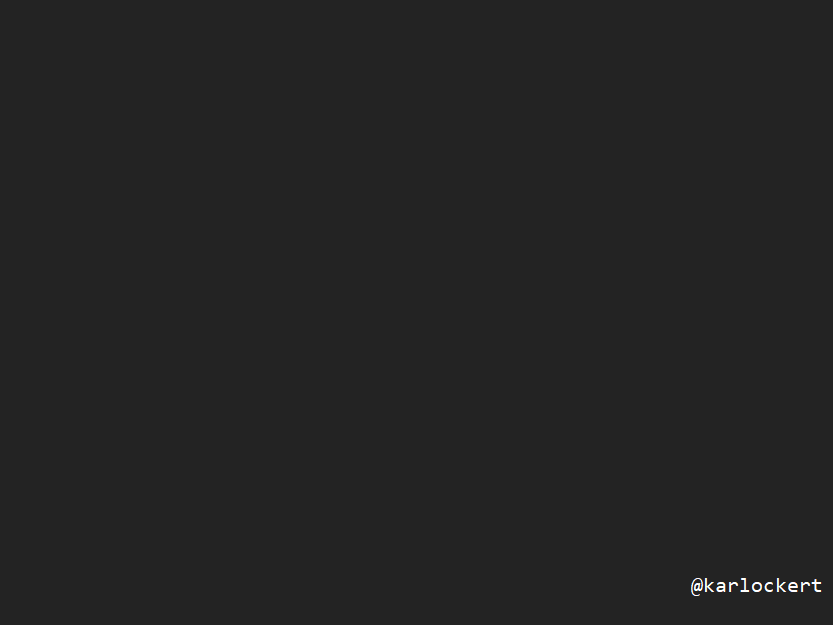
\includegraphics[height=\paperheight]{img/bakgrunn.png}};}

\begin{frame}[noframenumbering, plain]
	\begin{block}{\color{white}\textbf{\Large{
					%
					Superconductivity - BCS theory (1)
					%	
		}}}
		\vspace{-10pt}\rule{\textwidth}{0.5pt}
		\color{white}
		
	The Bardeen-Cooper-Schrieffer theory of superconductivity is the most celebrated microscopic theory describing the macroscopic phenomena of superconductivity. In this theory, an effective attractive potential between electrons in vicinity of the Fermi surface leads to the condensation of ``Cooper pairs'', reducing the free energy of the system. After some crude simplifications, a model Hamiltonian reads
		
	\end{block}
	{\large
		
		\begin{equation*} 
			\mathcal{H} = \sum_{k, \sigma}\varepsilon_kc_{k\sigma}^{\dagger}c_{k\sigma}  + \sum_{k, k'}V_{kk'}c_{k \uparrow}^{\dagger}c_{-k \downarrow}^{\dagger}c_{k'\downarrow}c_{k'\uparrow},
		\end{equation*}
	}
	
	\begin{block}{}
		\color{white}
		where $V_{kk'}$ is attractive in a thin shell close to the Fermi surface. This attractive potential can for instance be mediated by interacting with quantized lattice vibrations -- phonons. 
		
		
	\end{block}
	
	
\end{frame}




\begin{frame}[noframenumbering, plain]
	\begin{block}{\color{white}\textbf{\Large{
					%
					Superconductivity - BCS theory (2)
					%	
		}}}
		\vspace{-10pt}\rule{\textwidth}{0.5pt}
		\color{white}
		Since this Hamiltonian is quartic in fermion-operators, solving it exactly is very difficult. However, a mean field treatment is possible by letting $c_{-k\downarrow}c_{k\uparrow} = \ev*{c_{-k\downarrow}c_{k\uparrow}}$ + fluctuations, and the system might be solved. The self-consistent BCS gap-equation states
		
	\end{block}
	{
			\begin{align*}
					\Delta_k &= -\sum_{k'}V_{kk'}\Delta_{k'}\chi_{k'} \\
					\chi_{k} &= \frac{1}{\sqrt{\varepsilon_k^2 + \Delta_k^2}}\tanh(\frac{\beta}{2}\sqrt{\varepsilon_k^2 + \Delta_k^2}).
			\end{align*}

	}
	
	\begin{block}{}
		\color{white}
		This is a ``gap''-equation precisely because the condensation of Cooper pairs opens a gap $\Delta_k$ in the electronic excitation spectrum. A goal of modern physics is to find systems whose superconducting gap is as large as possible. 
		
		
	\end{block}
	
	
\end{frame}